\chapter[Stato dell'arte]{Stato dell'arte}
\label{chap:State-of-art}
Il Web Semantico è di natura un campo d'interesse interdisciplinare: oltre ai ricercatori informatici teorici, il cui coinvolgimento può essere riassunto nel miglioramento delle tecnologie e principi che costituiscono il Web Semantico, esistono contesti in cui si vorrebbe utilizzare questo nuovo paradigma Web come un semplice strumento, o estenderlo con nuove annotazioni semantiche. Per fare un esempio, quando verso il 2006 le ontologie nello stato in cui erano si sono dimostrate difficili da mantere e riutilizzare, si è sviluppato un insieme di principi per rendere più superficiale le annotazioni semantiche, chiamato \textit{Linked Open Data} \cite{hitzler2021review}. Essenzialmente l'organizzazione della conoscenza consisteva di grafi RDF che potevano essere collegati tra di loro qualora fossero presenti identificatori IRI (che identificano un nodo) in comune. In questo modo la collezione di tutti i grafi RDF collegati poteva essere inteso come un singolo grande grafo RDF, permettendo una maggiore integrazione e gestione dei dati rispetto alla gestione di un'ontologia. Negli ultimi due decenni, il Web Semantico si è arricchito di tecnologie, strumenti e metodologie grazie agli sforzi di ricercatori e aziende: contributi fondamentali dai campi del Natural Language Processing e Machine Learning  hanno permesso di sviluppare metodi per generare automatizzare (a volte in parte) compiti complessi, come derivare query SPARQL da domande in linguaggi naturale \cite{Evseev2020SPARQLQG, Zlatareva2021ProcessingNL, Hu2021NaturalLQ} oppure come la fusione di due ontologie partendo da testi che trattano del dominio descritto \cite{caldarolaMultiStrategyApproach} o ancora di aggiungere relazioni mancanti tra annotazioni semantiche \cite{discoveringmissingsemanticrelation, repairinghiddenlinks}. Nel 2012 Google ha lanciato il suo "knowledge graph", che si è diffuso rapidamente come tecnica di modellazione della conoscenza nel Web Semantico.
Le direzioni di ricerca 
\textbf{RISTRUTTURARE}

Seguendo le necessità degli utilizzatori, in breve, si è formata un'ampia collezione di letteratura e tecniche per ogni settore d'applicazione. 

La risultante letteratura di campi di applicazione disparati ha reso difficile trovare una terminologia comune su discipline del Web Semantico. In questo modo, è difficile comunicare fra ricercatori che partecipano attivamente allo sviluppo del Web Semantico

Anche se esistono termini non ambigui, dati dalla definizione di specifiche condivise come RDF \cite{RDFspecification}, 

Per i lettori interessati alle influenze e allo stato attuale del Web Semantico, \cite{hitzler2021review} è un'ottima e recente recensione che valuta aspetti sia negativi che positivi degli sviluppi del campo. Riferendoci alle problematiche evidenziate in \cite{hitzler2021review}, ci permettiamo di evidenziare quelle che sono state le più condivise nella nostra esperienza di introduzione nel Web Semantico:
\begin{description}
	\item[Uniformità della terminologia] Nell'introduzione della metodologia di sviluppo ontologico NeOn \cite{NeOn}, la scelta di introdurre un glossario dei processi e attività legati allo sviluppo di un'ontologia è a causa della ambiguità dei termini che descrivono processi come la fusione di ontologie, per cui a volte esistono multiple definizione usate allo stesso momento. Un altro esempio di una mancanza di disambiguazione nelle definizioni è il cosiddetto \textit{knowledge graph}, anche se è stato presentato per la prima volta 11 anni fa e sia tutt'ora largamente utilizzato. Ovviamente sforzi verso questo risultato sono stati proposti (in particolare, i lavori \cite{katsumi2018ontology, goy2015ontologies, NeOn} nel campo del riuso delle ontologie  e per i knowledge graph \cite{ehrlinger2016towards}). La ragione principale che dovrebbe spingere la comunità del Web Semantico nel trovare delle definizione comuni è che la disambiguazione dei termini funge da deterrente per la diffusione negli ambiti accademici e aziendali dei concetti e tecnologie del Web Semantico, oltre a facilitare l'apprendimento delle persone interessate a svolgere ricerca. Essendo un campo interdisciplinare, il Web Semantico può essere caratterizzato da dialoghi tra ricercatori specializzati in campi diversi. Senza una terminologia ben definita, non è possibile stabilire un campo comune per una corretta trasmissione della conoscenza fra gli esperti. Nella \autoref{sec:consolidamentoTerminologia} illustriamo i risultati della nostra indagine sulla definizione della terminologia, in particolare applicata alle ontologie e al loro riutilizzo.
	
	\item[Assenza di consolidamento] Intendiamo dire che anche se ci sono strumenti che utilizzano gli stessi standard, come RDF e OWL, non è detto che questi lavorino insieme l'uno con l'altro \cite{hitzler2021review}. Inoltre, diversità sui formalismi per rappresentare le ontologie e soprattutto l'assenza di un framework per la valutazione delle ontologie ostacola l'integrazione delle ontologie e il loro riutilizzo. Uno dei motivi principali per cui le ontologie sono utilizzati è il fatto di essere formalizzazioni di un dominio \textit{condivisa}, ma se limitiamo la riusabilità delle ontologie perdiamo uno dei suoi vantaggi caratteristici.
	
	\item[Scarso orientamento al riutilizzo] In \cite{whyareontologiesnotreused}, in cui gli autori comparano le tendenze di riutilizzo di ontologie contenute nella repository LOV (Linked Open Vocabularies) rispetto ai risultati ottenuti in lavori precedenti, viene rilevato che circa un terzo delle ontologie registrate non è stato possibile ottenerle correttamente. Le possibili cause rilevate dagli autori sono una mancanza di disponibilità di condividere (soprattutto da parte delle aziende) le ontologie sviluppate, assieme a una scarsa manutenzione orientata al riutilizzo di esse. Non tratteremo di questo tema in dettaglio, per approfondire vedere \cite{ontology2014summit, feasibilityStudy}.
	
\end{description}

\section{Consolidamento della terminologia}
\label{sec:consolidamentoTerminologia}

\textbf{frase molto evocativa trovata dentro NeOn \cite{NeOn}} \textsc{"il livello più basso della conoscenza in qualsiasi campo è la sua terminologia, senza la quale non è possibile una corretta trasmissione della conoscenza"}.


La letteratura di campi di applicazione diversi tra di loro ha reso difficile trovare una terminologia comune per discipline del Web Semantico come il campo dedicato al riutilizzo dell'ontologia. In questo modo, è difficile comunicare fra ricercatori di discipline di origine diverse che partecipano attivamente allo sviluppo del Web Semantico. Il riutilizzo delle ontologie è una disciplina attuale, in cui molti studiosi stanno proponendo metodologie innovative per facilitare o semi-automatizzare alcuni processi come l'allineamento o la fusione di due ontologie. Da questi sforzi sono nate metodologie di sviluppo di ontologie che incentivano il riutilizzo \cite{NeOn}, framework che combinano tecniche di integrazione e di NLP \cite{caldarolaMultiStrategyApproach} e algoritmi provenienti da paradigmi di rappresentazione di conoscenza paralleli alle ontologie \cite{FCA-Merge}. Eppure, per quanto si sforzi a fornire strumenti per facilitare questo riuso, non è stato definito ancora quando un'ontologia è riutilizzabile. Tra tutti i contributi incisivi citati precedentemente, e tanti altri per cui non c'è stato abbastanza tempo per leggerli, soltanto gli autori di \cite{katsumi2018ontology}, al meglio delle nostre conoscenze, hanno evidenziato questo problema fondamentale. Nel loro lavoro \cite{katsumi2018ontology}, i due autori sottolineano la mancanza di una definizione, di un limite esplicito e accettato di cosa sia il riutilizzo, e di cosa non sia. Questo porta ad ostacolare la sua diffusione. La mancanza di formalizzazione non riguarda soltanto la definizione delle discipline, ma anche sui concetti fondamentali su cui si basano. Un esempio che proviene dal campo dell'evoluzione ontologica1 è la definizione formale delle operazioni che vanno a modificare un'ontologia. Diversi sforzi verso una definizione comune e accettata dalla comunità di questa disciplina sono stati fatti. Ad esempio uno dei tentativi meno recenti, da noi considerato significativo, di Thomas Sindt \cite{...} di fornire un Abstact Data Type (ADT), ossia un tipo di dato che astrae dalla sua realizzazione. All'interno dell'ADT vengono definite delle operazioni su di esso che caratterizzano il suo significato. \cite{...} sfrutta questa astrazione per la rappresentazione delle ontologie basate su $\mathcal{ALC}$ (si vedano i concetti preliminari \autoref{sec:logicaALCOIQ}) tramite liste e le relative operazioni di modifica. La semantica delle operazioni è resa esplicita dalla definizione delle pre e post-condizioni per ognuna di esse. Questo consente di:
tracciare le versioni e il dominio d'interesse descritto;
risalire, per le modifiche lecite, alle versioni precedenti dell'ontologia andando ad invertire un numero arbitrario di operazioni.
Queste due operazioni, fondamentali nella gestione del ciclo di vita di un'ontologia, sarebbero state di facile implementazione attraverso l'ADT definito da Sindt, avvantaggiando le aziende interessate alle ontologie. Anche se non ha riscosso molto successo, l'idea di Sindt potrebbe essere riutilizzata attraverso i linguaggi funzionali, dato che le liste sono una delle strutture dati ricorsive manipolabili facilmente con essi. Continuare a spiegare perchè…
Da aggiungere parte intermedia per passare dall'articolo sopra, che parla di formalizzazione di operazioni, a quello sotto, che parla di comparazione tra ontologie e sistemi di tipo in chiave di ontology evolution.


\section{Riutilizzabilità delle ontologie}
\label{sec:OntoReuse}
La trasformazione delle ontologie è intrinseca negli obiettivi del Web Semantico. In una rete di conoscenza in continuo aggiornamento, l'aggiunta di nuovi dati può significare il cambiamento della modellazione dei concetti del dominio d'interesse, che sia un'aggiunta o sia una sottrazione di questi. Il valore delle ontologie è anche dato dalla loro riusabilità: è relativamente facile estenderle, aggiungendo nuovi concetti, oppure utilizzarle per generarne delle nuove basi di conoscenza. Il riutilizzo delle ontologie promuove l'interoperabilità delle fonti di dati e facilita il processo di creazione di nuove ontologie e l'integrazione dei dati, ed è fortemente legato ad altri processi di ingegneria delle ontologie.
\subsection{NeOn: una metodologia basata sul riutilizzo di ontologie}
La nascita di metodologie di sviluppo per ontologie durante gli ultimi due decenni ha portato alla considerazione del processo di creazione di un'ontologia come un'attività ingegneristica delle ontologie. \cite{iqbal2013analysis} è un ottimo punto di partenza per avere una panoramica introduttiva dei principali tool e metodologie per lo sviluppo di ontologie. Oltre che definire delle linee guida e scenari d'uso, questi approcci permettono al tempo stesso di esplicitamente definire fra un grande numero di ontologie meta-relazioni  come l'allineamento, la mappatura \cite{choi2006Mapping} o dipendenza, creando una \textit{rete ontologica}. Queste relazioni possono essere usate come base per il riutilizzo di ontologie relazionate in uno di questi modi. La tendenza attuale, infatti, è quella di sviluppare un'ontologia partendo da esistente risorse di conoscenza, in particolare da ontologie che descrivono un dominio genericamente vicino a quello d'interesse o parte di esso, e specializzarlo o estenderlo per raggiungere la realtà modellata desiderata.

NeOn \cite{NeOn} è stata una delle prime metodologie a fornire un framework per sviluppare un'ontologia e contemporaneamente una rete attorno ad essa. L'obiettivo di NeOn è quello di accelerare la costruzione di ontologie e reti ontologiche sfruttando specialmente il riutilizzo delle risorse di conoscenza disponibili, che siano o no ontologie. Questa metodologia è basata su 4 componenti fondamentali:
\begin{enumerate}[i.]
	\item un glossario di processi e attività;
	\label{itm:glossario}
	\item 9 scenari per costruire ontologie;
	\label{itm:scenari}
	\item due modelli per gestire il ciclo di vita di un'ontologia;
	\item un insieme di linee guida normative sulla modalità di svolgimento dei processi e attività.
\end{enumerate}
Come già detto in precedenza, il glossario (si veda \autoref{fig:NeONglossary}) definisce con precisione (anche se in linguaggio naturale) i processi e le attività che campo dell'ingegneria delle ontologie possono essere soggetti a multiple definizioni o ambigue. In questo, l'utilizzatore di questa metodologia non deve preoccuparsi di cercare il significato dei termini, in questo modo rendendo NeOn anche adatta ai principianti dello sviluppo delle ontologie. I termini inclusi nel glossario si riferiscono ad attività e processi, ossia rispettivamente azioni da svolgere, dettagliate anche attraverso la specifica dei documenti di input e il suo output, e gruppi di attività. 

\begin{figure}
	\centering
	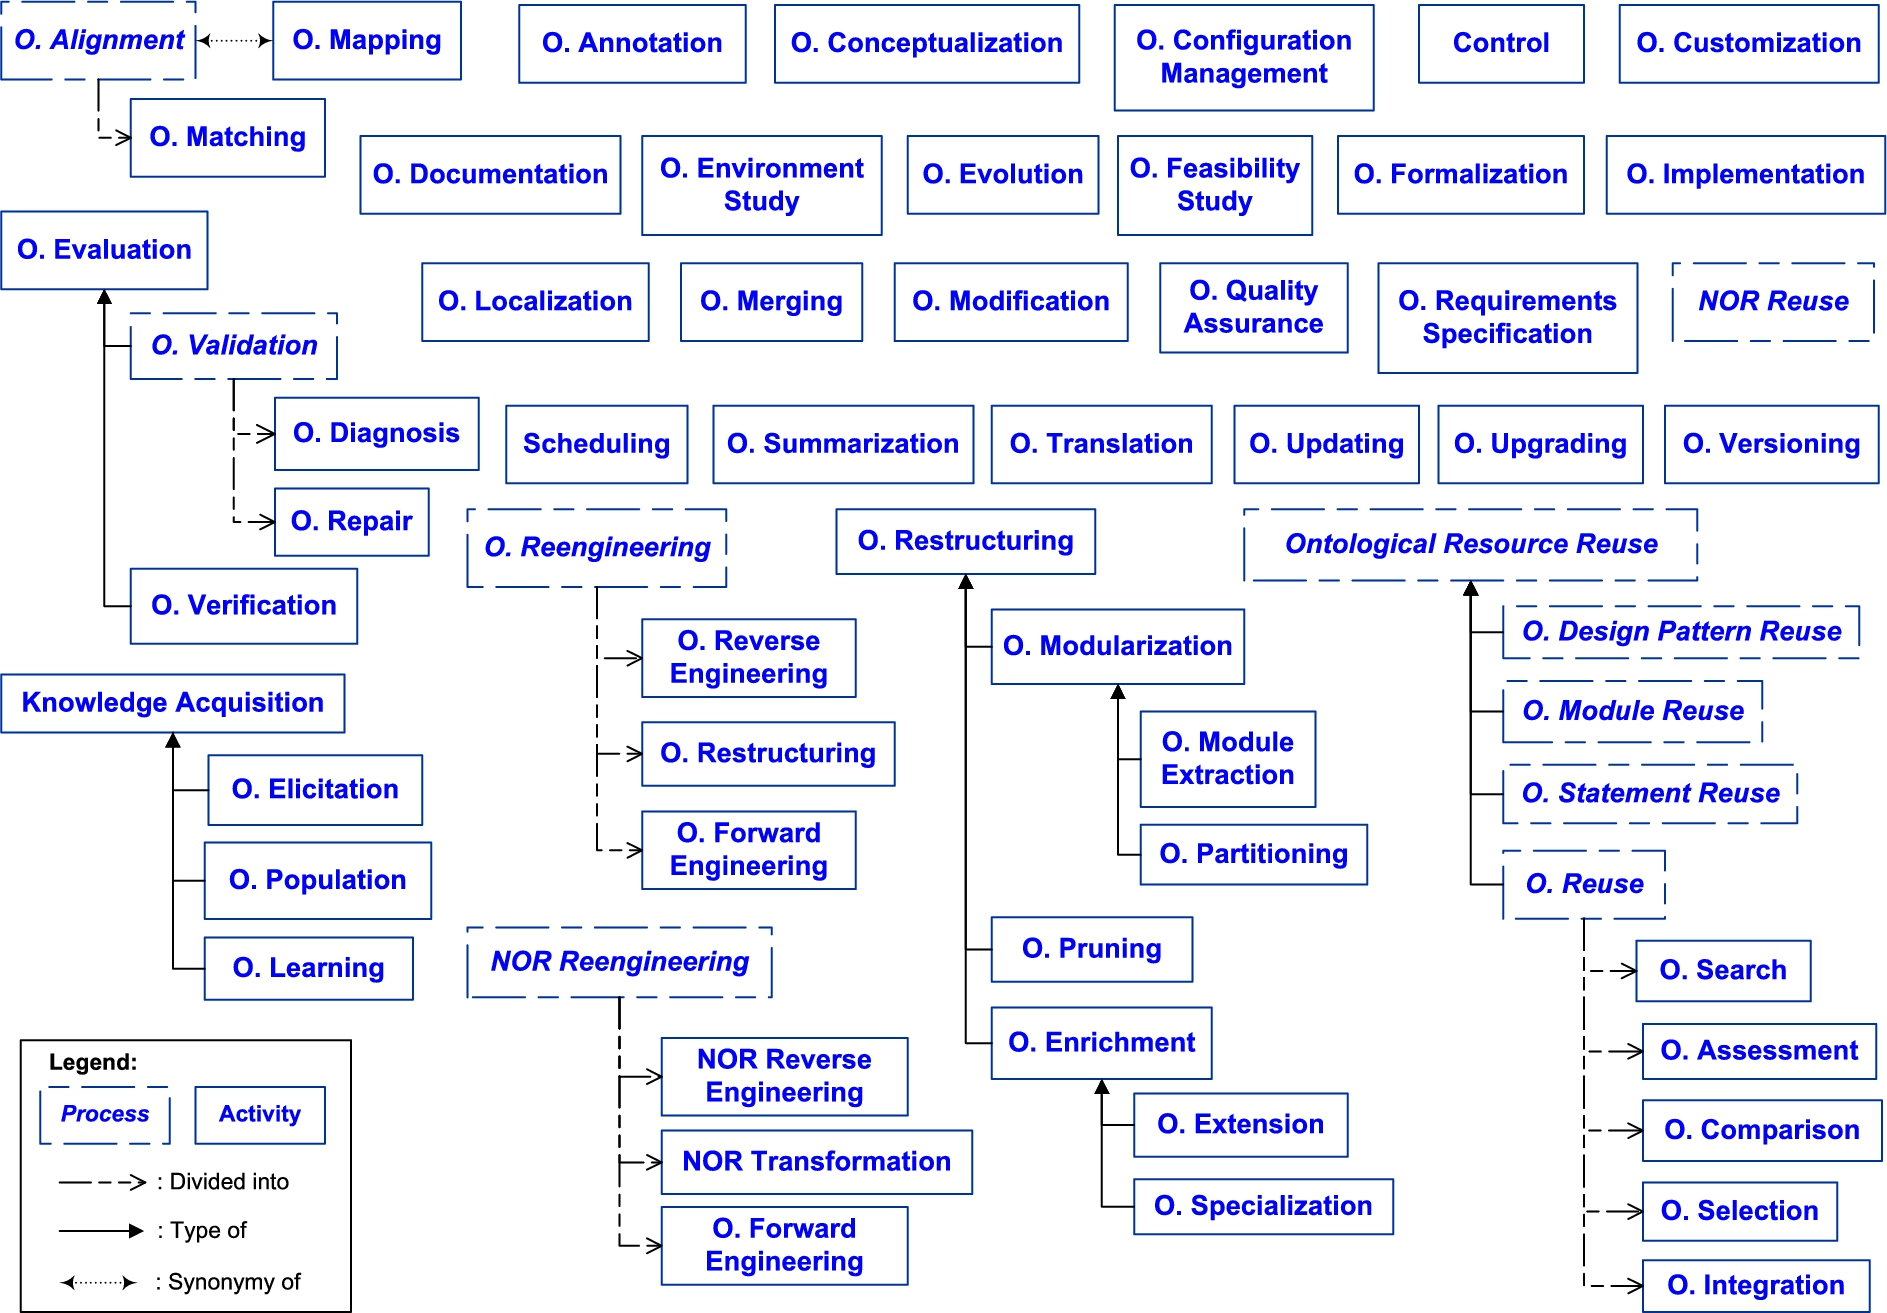
\includegraphics[scale=0.8]{pictures/NeOn-Glossary.jpg}
	\caption{glossario NeOn \cite{NeOn} di processi e attività.}
	\label{fig:NeONglossary}
\end{figure}

Gli scenari sono un altro punto forte della metodologia, permettendo di coprire flessibilmente gran parte degli scenari comuni che possono accadere durante lo sviluppo di un'ontologia, come ad esempio la ristrutturazione delle ontologie da riutilizzare, e potrebbero richiedere integrazione da parte di Ontology Design Patterns \cite{ODP} e/o altre risorse non ontologiche. Piuttosto che ripetere tutti gli scenari, ci concentriamo su quelli in cui il focus principale è il riutilizzo di ontologie, puntando al lettore a possibili riferimenti utili per eseguire una determinata attività caratteristica dello scenario.
\subsubsection*{Scenario 3: riutilizzare ontologie}
\label{sec:Scenario3}
Questo scenario è applicabile quando gli sviluppatori hanno accesso a ontologie che coprono, anche in parte, il dominio d'interesse dell'ontologia (o rete di ontologie) in sviluppo. Possiamo notare che le reti di ontologie fondamentali per NeOn leggendo il suggerimento presente all'inizio di ogni scenario. Ad esempio, in questo scenario, "\textsl{se l'obiettivo è quello di creare una rete d'ontologie, gli sviluppatori dovrebbero esplicitare le meta-relazioni (per esempio, \texttt{useImports} o \texttt{isReusing}) per modellare tale riuso}" \cite{NeOn}. Lo scenario prosegue e, facendo riferimento al processo di \textit{Ontological Resource Reuse} in \autoref{fig:NeONglossary}, suggerisce allo sviluppatore di svolgere le attività di \textit{ricerca} delle risorse, \textit{valutazione} dei risultati in base a criteri che indichino la vicinanza del dominio dell'ontologia trovata rispetto alla realtà d'interesse da rappresentare, \textit{comparazione} fra le ontologie per stabilire un ranking, \textit{selezione} delle migliore risorse rispetto alla realtà d'interesse e infine \textit{integrazione} di esse. Diversi riferimenti possono essere forniti interessati ad approfondire le attività citate sopra. In particolare sull'attività di ricerca di ontologie, sono stati sviluppati servizi di ricerca per trovare informazioni basate su RDF, primo fra tutti Swoogle \cite{swoogle}. Un search engine consigliato per questa attività è Watson\footnote{\url{http://watson.kmi.open.ac.uk/WatsonWUI/}} \cite{watson}, che non cerca di indicizzare tutti i documenti del Web semantico, ma si concentra specificamente sulle ontologie Web. Inoltre, fornisce alcuni metadati aggiuntivi sulle ontologie, come l'espressività degli assiomi ed eventualmente alcune recensioni.

Approfondimenti sulle attività non menzionate dell'Ontology Reuse e altri approcci al riuso delle ontologie possono essere trovati in \cite{carriero2020OntoReuse, caldarolaMultiStrategyApproach, ontologyEvaluation} e la loro bibliografia.
\subsubsection*{Scenario 4: riutilizzare e reingegnerizzare ontologie}
Questo scenario viene applicato quando i risultati delo Scenario 3 non sono utilizzabili nello stato in cui sono. Oltre al processo di \textit{riutilizzo di ontologie}, è necessario allora eseguire attività come il \textit{Reverse Engineering}, \textit{Restructuring}, che consiste nel correggere e riorganizzare il dominio d'interesse in un modello concettuale per poi rilevare le informazioni mancanti, e \textit{Forward Engineering}. Per questi scopi, uno sviluppatore di ontologie che incorre in questo scenario potrebbe beneficiare di editor di ontologie come Prot\'eg\'e \cite{protege} e (f OWL) \cite{fOWL} che permettono agli utenti di manipolare visivamente, ispezionare, sfogliare, codificare le ontologie, supportando lo sviluppo e la loro manutenzione \cite{alatrish2013comparison}. Esiste, inoltre, un ambiente di sviluppo apposta per NeOn, NeOn Toolkit \cite{NeOnToolkit}, più appropriato per ontologie di grandi dimensioni e attività di riutilizzo come integrazione (tipica appunto di NeOn).

\subsubsection*{Scenario 5: riutilizzare e fare merging fra ontologie}
Questo scenario dipende dall'obiettivo finale dello sviluppatore. In ogni caso, per poter considerare questo scenario, è necessario che ci siano diverse ontologie esistenti dallo stesso dominio che possono essere selezionate per il riuso (Scenario 3). Se lo sviluppatore vuole creare una nuova ontologia \textit{allineando} e facendo \textit{merging} due o più ontologie esistenti. Se invece volesse optare per stabilire una \textit{mappatura} o \textit{allineamento} fra le risorse esistenti selezionate per creare una rete di ontologie, lo scenario diventa semplice, trasformandosi nella definizione di meta-relazioni come \texttt{useImports} o \texttt{hasMapping}.

\cite{choi2006Mapping, carriero2020OntoReuse} ci aiutano ancora una volta con le definizioni, definendo \textit{ontology merging} come il processo in cui singoli concetti, assiomi e affermazioni di ontologie "sorgenti" vengono fusi insieme in un nuovo modello. Le ontologie originali hanno domini simili o sovrapposti, ma sono diverse e non revisioni della stessa ontologia. Sono necessarie attività di normalizzazione per confrontare uniformemente i concetti rappresentati da un'ontologia rispetto ad un'altra.

Il processo di \textit{mapping} è 


\subsection{Cosa si intende per riutilizzo nella letteratura}
Tra le poche definizione di riutilizzo di un'ontologia la più completa, seppur informale, può essere considerata "il processo in cui la conoscenza (ontologica) disponibile viene utilizzata come input per generare nuove ontologie" (tradotto da \cite{...}). Carriero et. al. \cite{...} danno un ottimo sguardo d'insieme sullo stato dell'arte, benefici, lacune e criticità dei vari approcci al riutilizzo di ontologie, dando un'analisi completa per i lettori interessati ad approfondire.
Esistono due strategie principali per il riutilizzo di ontologie: 
Il riuso diretto, che può essere portato avanti tramite l'assioma owl:imports, che importa intere ontologie, oppure tramite la sola inclusione di termini già definiti (facendo riferimento all'ontologia sorgente tramite rdfs:isDefinedBy). Nel primo approccio, le informazioni espresse dalle ontologie riutilizzate sono incluse nella nuova ontologia, mentre nel secondo il compito di chiarire la semantica dei termini è "delegata" all'ontologia riutilizzata.
Il riuso indiretto fa sì che i termini presi da ontologie esistenti si comportino da contesto (o template) per la definizione dei nuovi termini o proprietà della nuova ontologia, permettendo di allinearli semanticamente attraverso assiomi come rdfs:subClassOf o owl:equivalentProperty.
Per chiarire il punto 2, il processo di allineamento di ontologie si basa sulla creazione di riferimenti fra due ontologie. Questo permette di mantenere separate le ontologie ma di restare coerenti fra di loro. \cite{...}
Per generare un ontologia prendendo come base altre basi di conoscenza, si sono diffusi principalmente due metodi:
Ontology integration (anche detto modular composition): il processo di generazione di un'unica ontologia su un argomento da due o più ontologie esistenti e diverse su argomenti diversi. I diversi argomenti delle diverse ontologie possono essere essere correlati \cite{...}. Viene chiamato composizione modulare perché le ontologie "sorgenti" non trattano (solo) dello stesso argomento che stiamo cercando di descrivere con l'ontologia "risultante".
Ontology merging (anche detto fusion): processo in cui singoli concetti, assiomi e affermazioni di ontologie "sorgenti" vengono fusi insieme in un nuovo modello. Le ontologie originali hanno domini simili o sovrapposti, ma sono diverse e non revisioni della stessa ontologia. Sono necessarie attività di normalizzazione per confrontare uniformemente i concetti rappresentati da una base di conoscenza rispetto ad un'altra. \cite{.., ..}
\subsection{Problemi}
Scarso orientamento al riutilizzo In \cite{...}, in cui gli autori comparano le tendenze di riutilizzo di ontologie contenute nella repository LOV (Linked Open Vocabularies) rispetto ai risultati ottenuti in lavori precedenti, viene rilevato che circa un terzo delle ontologie registrate non è stato possibile ottenerle correttamente. Le possibili cause rilevate dagli autori sono una mancanza di disponibilità di condividere (soprattutto da parte delle aziende) le ontologie sviluppate, assieme a una scarsa manutenzione orientata al riutilizzo di esse.
Aggiungere altri, riconsultare Carriero e Choi
Formalizzazione della terminologia
Il riutilizzo delle ontologie è ancora un problema attuale, su cui molti ricercatori stanno trovando modi per sfruttare dei metodi provenienti da campi differenti (es. scienze cognitive, NLP e machine learning). Da questi sforzi sono nate metodologie di sviluppo di ontologie che incentivano il riutilizzo \cite{...},framework che combinano tecniche di integrazione e di NLP \cite{...} e algoritmi provenienti da paradigmi di rappresentazione di conoscenza paralleli alle ontologie \cite{...}. Tra tutti i contributi significativi citati, e tanti altri per cui non c'è stato tempo di leggere, soltanto Megan Katsumi e Michael Grüninger, al meglio delle nostre conoscenze, hanno evidenziato un problema fondamentale inerente a questo campo. Nel loro lavoro \cite{...}, i due autori sottolineano la mancanza di una definizione formale, di un limite esplicito e accettato di cosa sia il riutilizzo, e di cosa non sia. Questo porta ad ostacolare la sua diffusione. La mancanza di formalizzazione non riguarda soltanto la definizione delle discipline, ma anche sui concetti fondamentali su cui si basano. Un esempio che proviene dal campo dell'evoluzione ontologica1 è la definizione formale delle operazioni che vanno a modificare un'ontologia. Diversi sforzi verso una definizione comune e accettata dalla comunità di questa disciplina sono stati fatti. Ad esempio uno dei tentativi meno recenti, da noi considerato significativo, di Thomas Sindt \cite{...} di fornire un ADT2 per la rappresentazione delle ontologie basate su ALC1 tramite liste e le relative operazioni di modifica. La semantica delle operazioni è resa esplicita dalla definizione delle pre e post-condizioni per ognuna di esse. Questo consente di:
tracciare le versioni e il dominio d'interesse descritto;
risalire, per le modifiche lecite, alle versioni precedenti dell'ontologia andando ad invertire un numero arbitrario di operazioni.
Queste due operazioni, fondamentali nella gestione del ciclo di vita di un'ontologia, sarebbero state di facile implementazione attraverso l'ADT definito da Sindt, avvantaggiando le aziende interessate alle ontologie. Anche se non ha riscosso molto successo, l'idea di Sindt potrebbe essere riutilizzata attraverso i linguaggi funzionali, dato che le liste sono una delle strutture dati ricorsive manipolabili facilmente con essi. Continuare a spiegare perchè…
Da aggiungere parte intermedia per passare dall'articolo sopra, che parla di formalizzazione di operazioni, a quello sotto, che parla di comparazione tra ontologie e sistemi di tipo in chiave di ontology evolution.


\section{Ontologie e sistemi di tipo}
Nell'approfondire le ontologie si può pensare di paragonarle ai sistemi di tipi dei linguaggi di programmazione. La similarità che il lettore potrebbe scorgere deriva dal fatto che le ontologie, nel contesto del Web Semantico, hanno lo scopo di raggruppare sotto diversi insiemi, chiamati \textit{concetti}, i nodi dei grafi RDF. Riprendendo l'esempio \eqref{eq:T1.1} della \autoref{sec:KB}, se una tripla descrive che il nodo \textsl{bob} sia in relazione hasName con un altro valore, allora automaticamente possiamo dire \textsl{bob} che appartiene all'interpretazione del concetto Person. Prima di considerare come questo si potrebbe tradurre nella terminologia dei sistemi di tipi, ricordiamo la definizione comunemente accettata di un sistema di tipi \cite{pierceTypesBook}:
\begin{definition}
	Un sistema di tipi è un metodo sintattico trattabile, in grado di dimostrare l'assenza di determinati comportamenti nei programmi mediante la classificazione di espressioni fatta in base alla natura dei valori che esse elaborano.
\end{definition}
\noindent
In altre parole, esso raggruppa espressioni che producono valori simili in \textit{insiemi}, chiamati \textit{tipi}, e permette di stabilire quando un valore è permesso oppure no attraverso delle \textsl{regole di derivazione}. Riprendendo l'esempio precedente, allora, in un sistema di tipi potremmo rappresentare la stessa cosa aggiungendo una regola di derivazione per un termine che abbia la stessa proprietà di essere in relazione \textsl{hasName} con un altro valore.\\
In effetti, questa confronto fra ontologie e la parte dichiarativa di un programma, in particolare il sistema di tipi non è nuova \cite{moten2015SWTypeSystem, despeyroux2008evolution}, ma non ha nemmeno suscitato l'interesse dei ricercatori del Web Semantico, ad eccezione di alcuni autori che già operano nelle discipline teoriche dell'informatica applicate \cite{dapoigny2011typetheoryKR, leinbergerphdthesis, ciobanu2016typeFoundationforRDFS}. Una domanda, ancora senza interrogativo, è la motivazione dietro a questo scarso interesse.
In \cite{despeyroux2008evolution} il confronto proposto tra un'ontologia e un sistema di tipi è particolarmente interessante per le conclusioni tratte. Per rafforzare questa comparazione, viene affrontata l'analisi delle modifiche svolte durante l'evoluzione di un'ontologia, relazionandola con il processo di type-checking tipico dei sistemi di tipi.

\begin{figure}
	\begin{minipage}[t]{0.45\textwidth}
			\textbf{Concepts}: \textit{Person, Trainee,\\
			PhdStudent, Manager, Researcher,\\
			Director, Team,
			Project;}
			\begin{align}
			\textit{Researcher}\ &\text{is-a}\ \textit{Manager};&\\
			\textit{Director}\ &\text{is-a}\ \textit{Manager};&\\
			\textit{Manager}\ &\text{is-a}\ \textit{Person};&\\
			\textit{PhdStudent}\ &\text{is-a}\ \textit{Person};&\\
			\textit{Trainee}\ &\text{is-a}\ \textit{Person};&
			\end{align}
			
			\textbf{Properties}: work, manage;\\
			Person work Team;\\
			Manager manage Project;\\

		\textbf{Semantic annotations}\\
			(r1 work v1) (r1 type \textit{Person})\\
			(r2 work v2) (r2 type \textit{PhdStudent})\\
			(r3 work v3) (r3 type \textit{Manager})\\
			(r4 manage v4) (r4 type \textit{Manager})\\
			(r5 work v5) (r5 type \textit{Researcher})\\
			(r6 manage v6) (r6 type \textit{Researcher})\\
			(r7 work v7) (r7 type \textit{Director})\\
			(r8 manage v8) (r8 type \textit{Director})\\

	\end{minipage}
	\hspace{0.05\textwidth}
	\begin{minipage}[t]{0.45\textwidth}
		
			\textbf{Types}: \textit{Person}, \textit{PhdStudent}, \textit{Trainee}, \textit{Manager}, \textit{Researcher},\textit{Director}, \textit{Team}, \textit{Project} : Type;
			\begin{align}
			PhdStudent &\le Person;\\
			Trainee &\le Person;\\
			Manager &\le Person;\\
			Researcher &\le Manager;\\
			Director &\le Manager;
		\end{align}
			work : \textit{Person} $\to$ \textit{Team};\\
			manage : \textit{Manager} $\to$ \textit{Project};\\\\\\
			\textbf{Typing relations}\\
			r1 : \textit{Person};\\
			r2 : \textit{PhdStudent};\\
			r3, r4 : \textit{Manager};\\
			r5, r6 : \textit{Researcher};\\
			r7, r8 : \textit{Director};\\
			v1, v2, v3, v5, v7 : \textit{Team};\\
			v4, v6, v8 : \textit{Project};\\
	\end{minipage}
	\captionsetup{justification=Centering}
	\caption{confronto tra una dichiarazione di un'ontologia RDFS (dx) con un sistema di tipo (sx) in cui $\le$ è una relazione di sottotipo}
	\label{fig:confrontotypesystem}
\end{figure}
\noindent
Usando un'ontologia RDFS banale ma esemplificativa, \cite{despeyroux2008evolution} mostra che l'eventuale rimozione di  alcune definizioni di concetti dal T-Box porta le loro istanze presenti nelle annotazioni semantiche (asserzioni A-Box, vedi \autoref{def:ABox}) a rendere inconsistente l'intera annotazione rispetto all'ontologia modificata. Per fare in modo che le annotazioni rimangano consistenti alla base di conoscenza, è necessario individuare quelle inconsistenti e agire su esse.
In \autoref{fig:confrontotypesystem} è possibile vedere l'idea di \cite{despeyroux2008evolution}: se fosse possibile considerare i concetti definiti nell'ontologia come tipi, le relazioni "is-a"\footnote{ricordiamo che in OWL questo si esprime attraverso GCI, assiomi del tipo $C \sqsubseteq D$, con C e D concept expressions} tra i concetti come particolari relazioni di sottotipo e le proprietà come funzioni tra elementi tipati, sarebbe allora possibile trattate le annotazioni semantiche \code{t type \textit{Concept}} come asserzioni di tipo dell'elemento t. Le altre annotazioni sarebbe semplici termini per cui basta dimostrare controllare che i tipi del dominio e codominio della proprietà siano rispettati rispetto alla definizione nell'ontologia. Ad esempio, se abbiamo un'annotazione \code{t work s}, perchè questa sia consistente all'ontologia (sistema di tipi) è necessario che valgano $\text{t}: Person$ e $\text{s}: Team$. Per dimostrare la consistenza di entrambe le tipologie di annotazioni semantiche sarebbe quindi necessario, perchè questo confronto fra ontologia e sistemo di tipi valga, dimostrare la verità di queste relazioni di tipo, che è proprio quello che fa l'algoritmo di type-checking. Inoltre, se si utilizzasse un algoritmo di type inference \cite{cardoneTypeInference, martellimontanaritypeinference}, ossia un algoritmo per derivare automaticamente le  relazioni di tipo, in base alla definizione di \code{work} e \code{manage} si potrebbero derivare alcune delle relazioni di tipo dichiarate, come ad esempio $\text{r1} : \textit{Person}$, come farebbe proprio un'ontologia RDFS/OWL.\\
Data la similarità delle ontologie con i sistemi di tipi, \cite{despeyroux2008evolution} arriva alla conclusione che cercare di sfruttare tecniche tipiche dei sistemi di tipi come \textit{polimorfismo}, \textit{overloading} e \textit{parametri di tipo} (per approfondire questi e altri termini consultare \cite{pierceTypesBook}) per creare linguaggi ontologici più espressivi e modulari beneficerebbe il campo della knowledge representation (KR). Questa intuizione è stata portata avanti dalle ricerche di Richard Dapoigny e Patrick Barlatier verso l'applicazione della teoria dei tipi, cioè lo studio dei sistemi di tipi, alla KR. L'approfondimento del loro lavoro richiederebbe però la definizione di conoscenze preliminari che non abbiamo il tempo di definire in questa tesi. Rimandiamo i lettori interessati agli articoli \cite{dapoigny2011typetheoryKR, dapoigny2012typetheoryKR} e alla loro dettagliata bibliografia.
Un aspetto fondamentale che differenzia un'ontologia dai sistemi di tipi è la frequenza della necessità di estensione. La trasformazione delle basi di conoscenza è intrinseca nella natura del Web Semantico, come spiegato nella \autoref{sec:OntoReuse}. Al contrario, l'estensione di un sistema di tipi nei linguaggi di programmazione è di solito dipendente dall'aggiunta di costrutti sintattici del linguaggio di programmazione \cite{pierceTypesBook}, evento molto più raro. Per raggirare questo problema, i linguaggi di programmazione moderni offrono costrutti sintattici per creare nuovi tipi di dato. Nei linguaggi object-oriented come Java questo equivale a definire nuove classi o interfacce, quindi ad esempio la definizione di un albero binario può essere rappresentato in questo modo:
\begin{minted}{java}
		public abstract class Tree {
			Tree left;
			Tree right;
			public boolean empty();
		}
		
		public class Branch extends Tree {
			int value;
		
			public int empty(){ return false; }
		}
		
		public class Leaf extends Tree {	
			public int empty(){ return true; }
		}
\end{minted}
Nei linguaggi funzionali questo stesso costrutto prende il nome di \textit{dichiarazione di tipo}:
\begin{minted}{haskell}
	data Tree Int = Leaf | Branch Int (Tree Int) (Tree Int)
	
	empty : Tree Int -> boolean
	empty Leaf = true
	empty _ = false
\end{minted}
L'essenza di questa dichiarazione è che si usa la parola chiave \code{data}, si dà il nome del tipo e un numero arbitrario di variabili di tipo. In questo caso, è necessario specificare \code{Int} per associare ad ogni nodo (che non sia una foglia) un valore intero. Seguono poi i valori (casi) che possono valere per gli elementi del tipo \code{Tree}: \code{Leaf} è il "caso base", una costante senza valore (è stata definita anche così nella classe Java). Il costruttore \code{Branch Int (Tree Int) (Tree Int)} è chiaramente ricorsivo, il che ci permette di costruire un albero binario profondo a piacimento. Un esempio di elemento appartenente al nuovo tipo \code{Tree} potrebbe essere \code{Branch 2 (Branch 1 Leaf Leaf) (Branch 3 Leaf Leaf)}.

Gran parte della letteratura sembra preferire i linguaggi object-oriented, in particolare Java, per sviluppare applicazioni e strumenti che utilizzano le tecnologie del Web Semantico. In effetti Java è un linguaggio di programmazione maturo, con una grossa comunità di sviluppatori e aziende che forniscono librerie e documentazione, nato oltretutto per sviluppare applicazioni che si interfaccino con il Web. Da oltre 10 anni, inoltre, è disponibile OWL API \cite{OWLAPI}, una libreria Java che espone un'insieme di procedure che consentono di creare, manipolare e serializzare ontologie OWL, oltre a parsificare e scrivere file OWL in diverse sintassi. Questa API facilita talmente tanto lo sviluppo della parte basata sulle ontologie che è ormai diventata una componente fondamentale di una vastità di tools e applicazioni, tra cui il reasoner con cui abbiamo implementato il calcolo di Leinberger nel \autoref{chap:Implementazione}, HermiT \cite{HermiTWhitepaper}. Anche Leinberger stesso, nell'implementazione in Scala della suo sistema \cite{leinbergerScalaImpl}, ha usato lo stesso reasoner. Il difetto principale dello sviluppo di software basato su ontologie rappresentate in Java è che i ragionamenti automatici sono eseguiti a run-time, cioè durante l'esecuzione del programma. Se incorrono errori a run-time riguardanti un'ontologia, come ad esempio una query SPARQL non abitata (vedere \autoref{sec:SPARQLIntro}), non c'è alcuna garanzia formale che il programma possa terminare dando il risultato desiderato \cite{leinbergerphdthesis}. Proponiamo, quindi, di sfruttare i sistemi di tipi statici in cui l'utilizzo dei tipi, controllati a tempo di compilazione, potrebbero essere una risposta ai problemi di efficienza per il controllo di certe proprietà che avrebbe senso controllare a priori, e/o nel caso di grandi quantità di dati.

\subsection{Ontologie e linguaggi funzionali}
In questa sezione, l'obiettivo della trattazione sarà di fornire una quanto più esaustiva indagine, nelle limite delle nostre capacità, sulla rappresentazione di ontologie nei linguaggi funzionali, così come evidenziare proposte di sistemi di tipi estesi in modo da integrare i costrutti logici delle ontologie basate su logiche descrittive.
L'editor di ontologie (f OWL) \cite{fOWL} scritto in un dialetto di LISP, Clojure, è presentato. Clojure è un linguaggio funzionale che compila con la Java Virtual Machine, in questo modo è altamento portabile. (f OWL) implementa la sintassi funzionale di OWL 2. Il risultato ottenuto vuole essere un'alternativa alla diffusa OWL API, scritta in Java, per quei programmatori di linguaggi funzionali interessati a l'ingegnerizzazione delle ontologie. Allo stesso tempo, promuove la lazy-evaluation dei linguaggi funzionali per semplificare la creazione e modifica di un'ontologia, come mostrato nella parte finale dell'articolo in cui vengono comparate le prestazioni di OWL API e (f OWL). Quest'ultima eccelle soprattutto nella creazione della Negation Normal Form (NNF), una pratica di normalizzazione approvata dalla comunità per andare a confrontare uniformemente l'espressività degli assiomi di classe di un largo numero di ontologie.

In questo articolo \cite{verifiableontologybasedcomputation}, le potenzialità di Haskell di implementare software corretto che ragioni su un'ontologia, in particolare della Basic Formal Ontology\footnote{\url{https://basic-formal-ontology.org/}}, sono discusse. Viene presentata una nozione di computazione basata sulle ontologie. In una parte significativa della comunità ontologica, questo concetto è associato alla dimostrazione automatica di teoremi. Gli autori introducono una nozione più ampia, che richiede che i dati di input, le trasformazioni e l'output siano coerenti con una determinata ontologia. Viene fornito un esempio che mostra come la gerarchia delle sottoclassi di un'ontologia possa essere utilizzata come vincoli di tipo in Haskell. Sebbene esistano generatori di codice OWL per linguaggi come Java, la traduzione in Haskell descritta nell'articolo fa un uso significativo del suo sistema di tipi espressivo per consentire la verifica a tempo di compilazione della concettualizzazione ontologica. Inoltre, a differenza dei linguaggi imperativi, per cui è difficile dimostrare formalmente che il calcolo sia corretto, completo e termini, in Haskell l'assenza di side effect, la dipendenza del risultato di una funzione solo dai suoi argomenti e la lazy-evaluation permettono di semplificare la verifica di questi caratteristiche per i programmi funzionali \cite{hugheswhyFPMatters}. L'articolo può essere considerato innovativo per due motivi:
\begin{enumerate}
	\item Presenta un'idea nuova, poiché non sembra esistere ancora una traduzione tipizzata dalle ontologie OWL-DL ai programmi Haskell.
	\item Avanza la proposta che potrebbe essere facile generare automaticamente il codice per rappresentare i vincoli di tipo da fornire al sistema di tipo di Haskell. In questo modo, l'evoluzione costante di un'ontologia non sarebbe affatto un problema per la manutenibilità del software che permette di ragionare sulla stessa.
\end{enumerate}


